\documentclass[]{ltjsarticle}
\usepackage{luatexja}
\usepackage[top=20mm, left=20mm, right=20mm, bottom=25mm]{geometry}
\usepackage{url}
\usepackage{newpxmath,newpxtext}
\usepackage{color}
\usepackage{amsmath}
\usepackage{graphicx}
\usepackage{listings} %日本語のコメントアウトをする場合jvlisting(もしくはjlisting)が必要
%ここからソースコードの表示に関する設定
\lstset{
  basicstyle={\ttfamily},
  identifierstyle={\small},
  commentstyle={\smallitshape},
  keywordstyle={\small\bfseries},
  ndkeywordstyle={\small},
  stringstyle={\small\ttfamily},
  frame={tb},
  breaklines=true,
  columns=[l]{fullflexible},
  numbers=left,
  xrightmargin=0pt,
  xleftmargin=3pt,
  numberstyle={\scriptsize},
  stepnumber=1,
  numbersep=1pt,
  lineskip=-0.5ex
}

\title{熱伝導方程式の数値的解法}
\author{森田~太郎}
\date{}

\begin{document}
	\maketitle
	\section{はじめに}
	熱伝導方程式に代表される偏微分方程式はコンピュータにおける数値計算によって計算されることが一般的である。
	ここでは比較的学習コストが低いと言われているPythonを用いて熱伝導方程式を解くことを目的とする。
	また従来はAnacondaを使うのがベストプラクティスとされていたが、Pythonをweb開発などの他の業務で使う際はそうではない場合が多いため本稿ではAnacondaを使わない
	\footnote{数値計算しかしない場合はベスト。AnacondaのnumpyはIntelCPUに最適化されている。}。

	\section{開発環境の構築}
	\subsection{Pythonのインストール}
	プログラミング言語Pythonのインストール方法を示す。
	既にAnacondaをインストールしている場合は次セクション「はじめのコード」まで呼び飛ばした方が良いかもしれない\footnote{Anacondaと純Pythonの共存はなにかと面倒が多い気がする(やったことないのでわからない)}
	\begin{enumerate}
		\item \url{https://www.python.org/downloads/}にアクセスし、「Download」ボタンからPythonインストーラーをダウンロードする。
		\item ダウンロード後にインストーラーを起動しPythonをインストール。
		\item \textcolor{red}{インストール時に「Add to PATH」にチェックを入れること(重要)}
	\end{enumerate}
	以上でプログラミング言語Pythonのインストールは完了した。

	\subsection{パッケージのインストール}
	Pythonだけでもプログラムを書くことはできるが、Pythonの素晴らしさは先人が作ってきたプログラムをライブラリとして使用できる点である。
	Pythonは科学技術計算に強いと言われているが、それはPythonには科学技術計算に必要な「Numpy、Scipy」といったライブラリやデータプロットの「Matplotlib」が使用できるからである。
	ここでは科学技術計算に必要なライブラリをインストールする。
	\begin{enumerate}
		\item windowsのスタートから「Windows Powershell」を開く(検索ウィンドウから探すと早い)。
		\item 「pip3 install matplotlib numpy scipy」と打ち込みEnterキーを押す。このときPythonインスートル時にパスを追加していないとエラーが出る。
	\end{enumerate}


	\subsection{Vusial studio codeのインストール}
	Python自体のインストールはここまでで完了しているが、プログラムの内容(スクリプト)を編集するアプリケーションを用意するのが良い。
	数あるエディタから今回は比較的導入しやすいVisual Studio Codeを紹介する。

	\begin{enumerate}
		\item \url{https://code.visualstudio.com/download}からインストーラーをダウンロードする。
		\item インストールする。
	\end{enumerate}
	以上でVisual Studio Codeのインストールは完了した。

	\subsection{Visual studio codeの設定}
	Visual Studio Codeは標準アプリのメモ帳と比較して以下のようなメリットがある。
	\begin{itemize}
		\item コードがシンタックスハイライトされており、可読性が向上している
		\item 括弧やコードが自動で補完される(自動補完機能)
		\item Visual Studio Code内でプログラムを実行できる
		\item デバック機能が付属している
	\end{itemize}
	またVisual Studio CodeはPythonに限らずほとんど全てのプログラミング言語を扱うことのできる汎用性に優れたアプリケーションである。

	Visual studio codeのインストールは以上で完了したが、Pythonを使うには若干の設定が必要である。

	\subsection{拡張機能のインストール}
	Visual studio code上でPythonを有効に使用するためには拡張機能をインストールする必要がある。
	\begin{enumerate}
		\item Visual studio codeのメニュー画面左側の「Extensions」をクリックし、検索ウィンドウに「Python」と入力しEnterキーを押す。
		\item 表一番上の拡張機能をインストールする(写真\ref{fig:vscode-extension}参照)
	\end{enumerate}
	これでVisual Studio Code上でPythonが使えるようになった。


	\begin{figure}
		\centering
		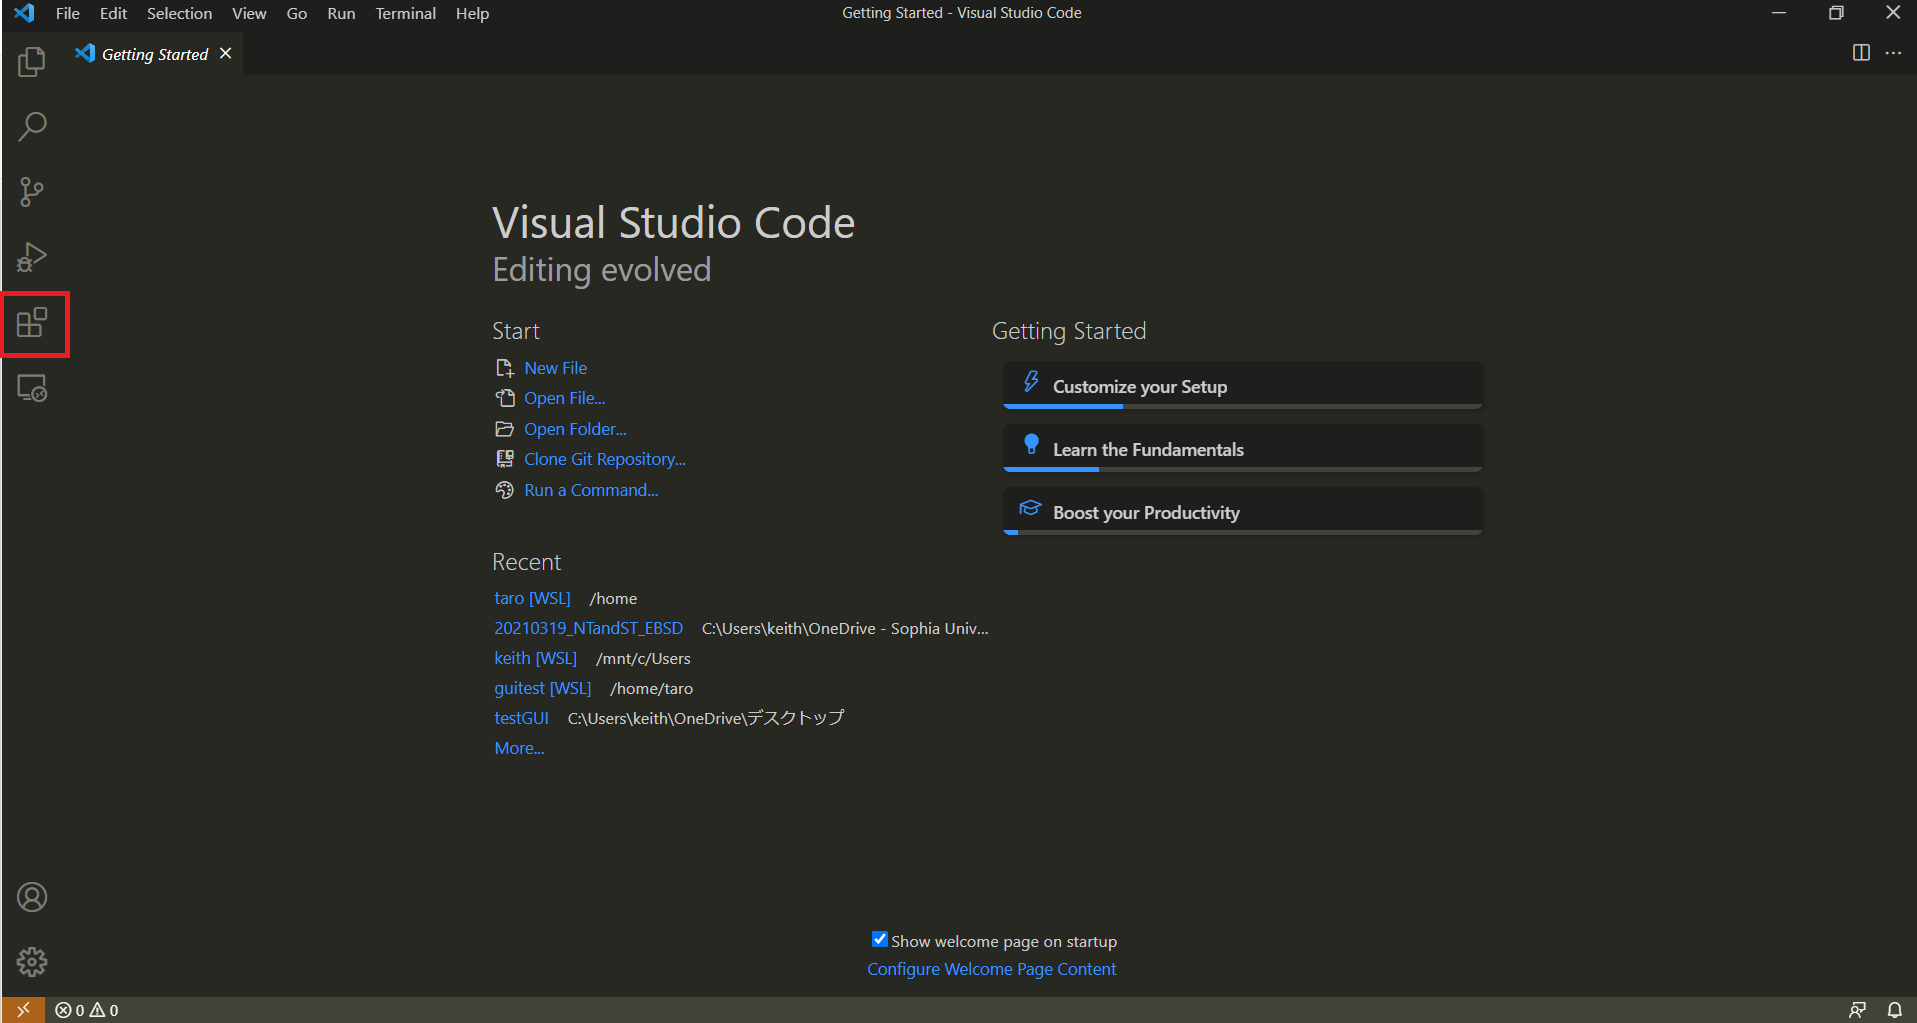
\includegraphics[width=0.9\linewidth]{figs/vscode1.png}
		\caption{Visual studio codeのメニュー画面}
		\label{fig:1}
	\end{figure}

	\begin{figure}
		\centering
		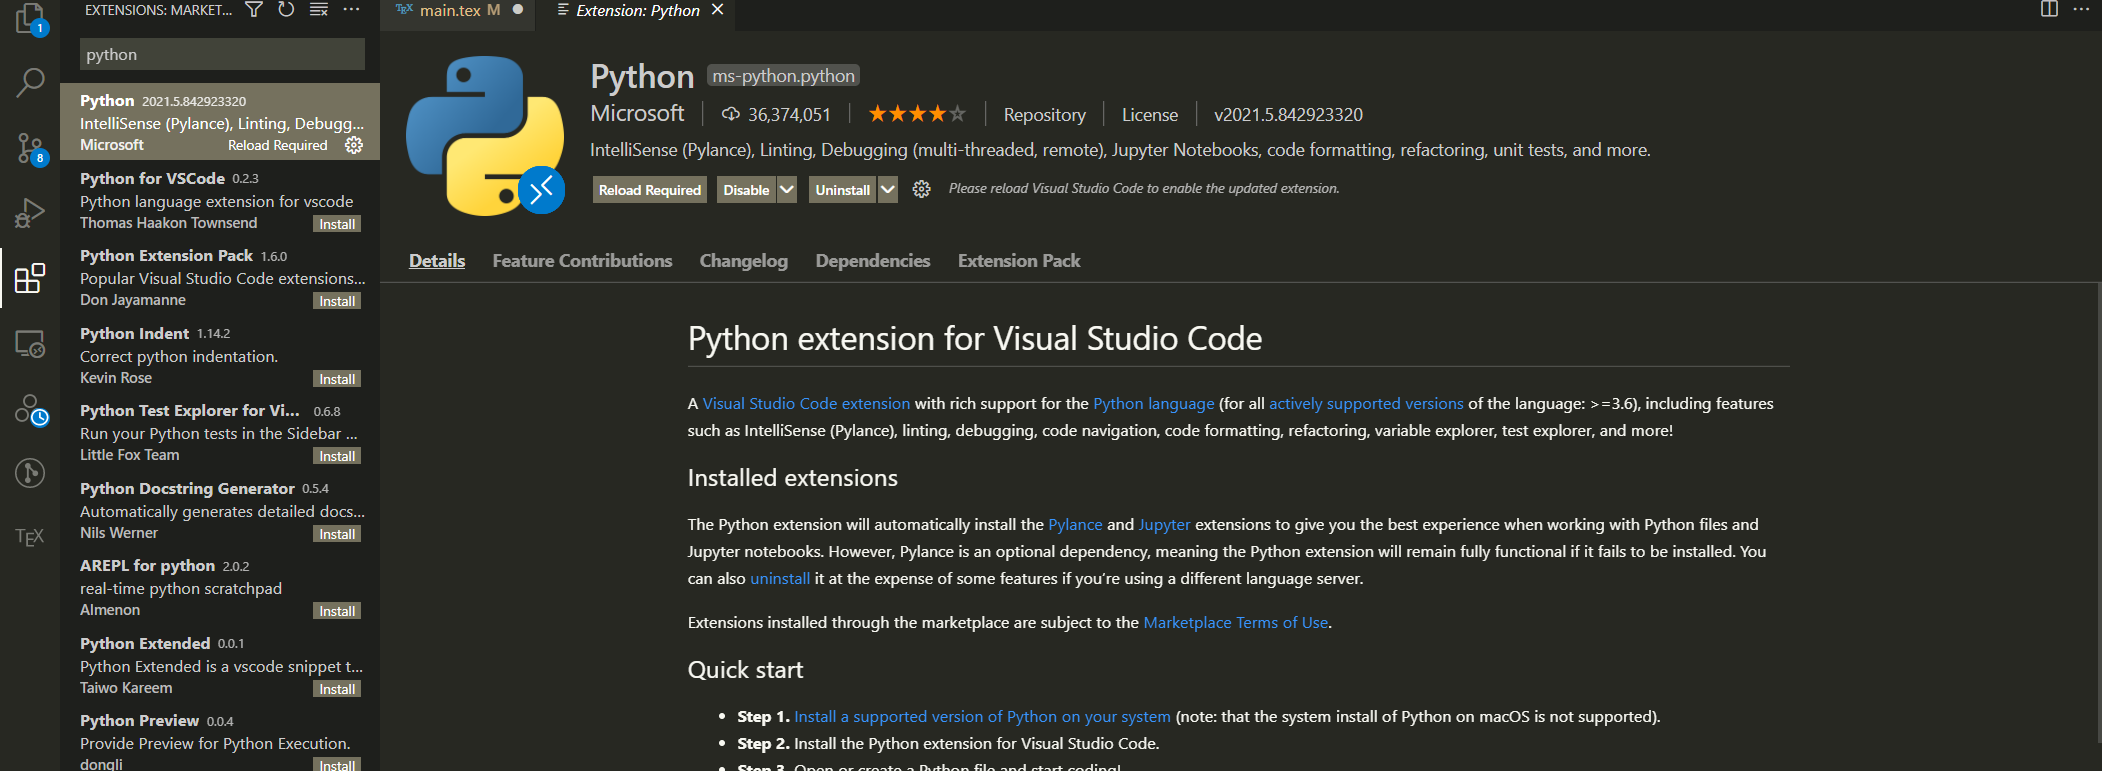
\includegraphics[width=0.9\linewidth]{figs/vscode2.png}
		\caption{Vscodeの拡張機能画面}
		\label{fig:vscode-extension}
	\end{figure}

	\section{はじめのコード}
	まず手始めに画面に「Hello world」と表示されるプログラムを書いてみる(プログラミング言語はまずHello worldから学習を始める)
	Visual Studio Code(以下Vscode)の左上「File」ー「New File」からファイルを新規作成する。
	新しくタブが開かれるのですぐに「File」ー「Save」でファイル名をつけて保存する。このときファイル名を「hello.py」とすること。
	一般的にファイルの「.」以降を拡張子と呼び、取り扱うアプリケーションやプログラミング言語によって異なる。
	Pythonファイルの拡張子は「.py」である。
	ファイルの拡張子を「py」としないとPython側でファイルを認識しないので注意する。
	ここではファイル名を「hello.py」として以下のコードを書いてみよう。

	\begin{lstlisting}[caption=hello.py,label=fuga]
		print("Hello world")
	\end{lstlisting}
	コードを書いたらファイルを保存し、VScode右上に表示されている緑色の矢印ボタン(再生ボタンみたいな)を押してコードを実行する。
	画面下にPowershellが開いてコードが実行されて、Hello worldと表示されただろうか?
	もしエラーが表示されている場合はエラー内容を読んで、コードをもう一度見直してみよう。
	直したら上記の手順で再度実行しよう。
	おめでとう!これで君はPythonを使えるようになった!

	\section{次のステップへ}
	画面にHello worldを出力するだけでは退屈なので、もう一つステップアップしたプログラムを書こう。
	ここでは科学技術計算らしく、numpyとmatplotlibを用いてSinプロットを行うプログラムを書く。
	以下にコードを示す。
	\begin{lstlisting}[caption=sin curve, label=sin]
		import numpy as np
		from matplotlib import pyplot as plt

		x = np.linspace(0, 10, 1000)
		y = np.sin(x)

		plt.plot(x, y)
		plt.show()

	\end{lstlisting}
	Sinカーブは出力されただろうか?
	次にコードについて説明する。
	1行目、2行目ではライブラリのインポートを行っている。
	ここでは数値計算ライブラリのNumpyとデータプロットライブラリのMatplotlibをインポートしている。
	4行目では0から10まで等間隔に1000分割した配列(ndarray)を作成している。
	Numpyを使わずにこの機能を実装すると割と大変だが、Numpyによって1行のコードで実現できる。
	5行目では作製したxを変数としてSinを適応した配列をyに代入している。
	7行目ではMaplotlibのplot関数を用いてx vs y(Sinカーブ)を出力している。

	このように数値計算ライブラリのNumpyを使うことで楽にSinカーブをプロットすることができた。

	\section{Pythonで数値計算の基礎知識}
	\subsection{変数}
	プログラミングでは「変数に値を代入する」という作業が多い。
	コードで書くと以下の通りである。
	\begin{lstlisting}{caption=variable, label=val}
		a = 1
	\end{lstlisting}
	これは「aという変数に1を代入する」を示す。
	我々は「a = 1」を目にすると「aは1に等しい!」と脊髄反射的に認識してしまうが、プログラミングの世界ではそうではなくあくまで「代入している」。
	言い換えれば「=」は「代入を示す演算子」である。

	変数についてさらに詳しく記す。
	コンピュータ上にはメモリというデータを保管する装置が存在する。
	これは「横に連なるロッカー」のような構造をしており、ロッカーの一つ一つにデータを格納することができる。
	このロッカーのようなものをアドレスというが、変数とはこの「メモリ上のあるアドレス」についた名前を指す。
	つまり「変数aに1を代入する」とは「メモリ上のあるアドレスにaという名前をつけてそこに1を格納する」ことである~(図\ref{fig:memory1}参照)。

	\begin{figure}
		\centering
		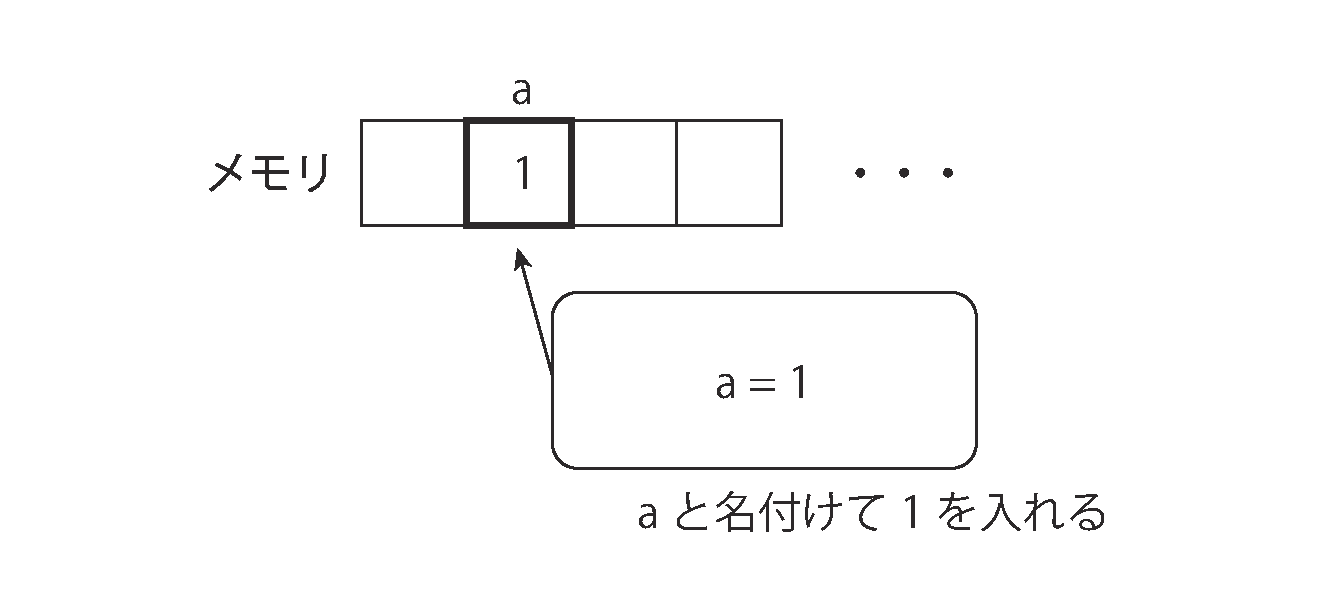
\includegraphics[width=0.8\linewidth]{figs/memory_explain1.pdf}
		\caption{メモリと変数の関係の定性的な説明}
		\label{fig:memory1}
	\end{figure}

	\subsection{配列}
	どのプログラミング言語にも「配列」といったデータを一括に扱う方法が存在する。
	前述した変数ではa = 1のように1つの変数につき1つのデータしか格納することができない。
	この場合、例えば時刻のようなデータを格納する場合は不便であるが、配列を使うことによって多数のデータを1つの変数として使うことができる。
	以下に配列をつかったコードを示す。
	\begin{lstlisting}[caption=array.py, label=array]
		x = [1, 2, 3]
		print(x)
	
	\end{lstlisting}
	上記コードを実行すると「[1, 2, 3]」が出力される。
	このように配列を用いることでxに1, 2, 3の値を一括して格納することができた。

	配列とメモリの関係を以下に示す。
	配列を作成するときはメモリ上で配列の大きさ分を確保し、その後に逐次1, 2, 3と代入する。
	つまり「a = [1, 2, 3]」ではまず配列の大きさである3マス分をメモリ上で確保しその領域をaと名付け、逐次1,2、3と代入する~(図\ref{fig:memory2}参照)。
	\begin{figure}
		\centering
		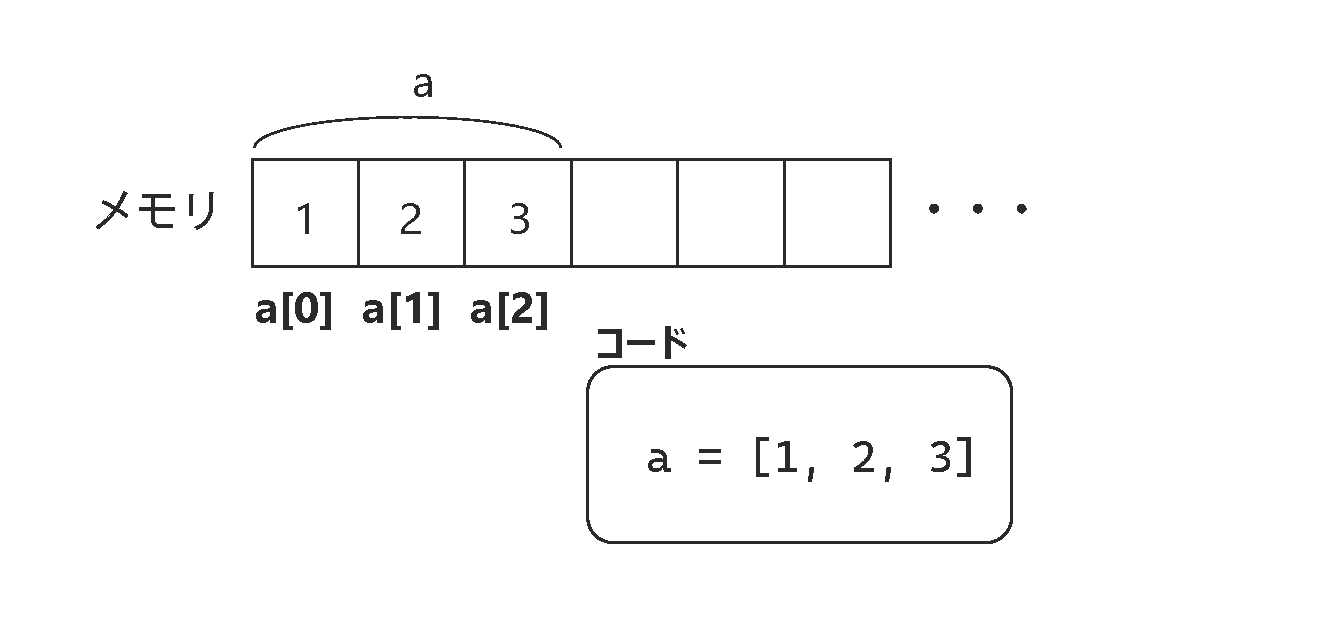
\includegraphics[width=0.8\linewidth]{figs/memory2.pdf}
		\caption{配列とメモリの関係の定性的な説明}
		\label{fig:memory2}
	\end{figure}

	実際に配列を用いて計算するには配列から要素を取り出す必要がある。
	例えば「xから1をとりだして、それに2を加えたい」といった処理を行うためにはxから1を取り出す必要がある。
	その処理を実現したコードを以下に示す。
	\begin{lstlisting}[caption=array.py, label=array2]
		x = [1, 2, 3]
		ans = x[0] + 2
	\end{lstlisting}
	配列の要素を取り出すときはa[0]のようにして数字で要素を指定する。
	この数字をインデックスというが、配列の$n$番目にある数値を取り出したい場合はインデックスとして$n-1$を指定する。
	ここで注意すべきなのはインデックスの開始番号は0からであるということである\footnote{多くのプログラミング言語ではこの仕様。Matlabは異なる。}。
	つまり1番目の要素を取り出したい場合はインデックスとして0を指定する。
	10番目の要素を取り出したい場合はインデックスとして9を指定する。

	またPythonでは配列に似た構造としてタプルやリストが存在するが、これらは混同しやすく混乱の元となるため本稿ではnumpyのndarrayを配列とする。
	numpyの配列ndarrayは以下のようにして定義することができる。
	\begin{lstlisting}[caption=numpyarray.py, label=ndarray]
	import numpy as np

	x = np.array([1, 2, 3])
	\end{lstlisting}

	\subsection{多次元配列}
	上述した配列はいわゆる1次元の配列である。
	特に数値計算では2次元以上の多次元配列を使う場合が多い。
	2次元配列の定義の仕方を以下に示す。
	\begin{lstlisting}[caption=2darray.py, label=2darray]
	import numpy as np

	x = np.array([[1, 2, 3], [4, 5, 6]])
	print(x)

	x1 = x[0, 0]
	print(x1)
	\end{lstlisting}
	行列$\begin{pmatrix} 1 & 2 & 3 \\ 4 & 5 & 6 \end{pmatrix}$が出力された。
	2次元配列の要素を取り出すにはx[i, j]とインデックスを2つ指定する。
	i、jはそれぞれ行、列に対応する。

	\subsection{制御構文}
	プログラミングをするメリットはなんだろうか?
	それは「退屈な繰り返し処理をパソコンに任せる」であると思う。
	ここではその繰り返し処理の基本について記す。

	Helloと10回出力する処理の実装を考えてみよう。
	ここまでの知識では以下のようなコードが考えられよう。
	\begin{lstlisting}[caption=hellloop.py, label=helloloop]
	print("hello")
	print("hello")
	print("hello")
	print("hello")
	print("hello")
	print("hello")
	print("hello")
	print("hello")
	print("hello")
	print("hello")
	\end{lstlisting}
	非常に退屈なコードである。
	なぜならば、あなたは「print("hello")」を数え間違えないように細心の注意を払って10回書かなければならないからである。
	これでは処理をコンピュータに任せる意味がない。
	コンピュータにこのような「退屈な繰り返し処理」を任せる方法を記す。
	\subsection{while構文}
	whileは「$\sim$する限り」という意味がある。
	プログラミングでもその意味の通りの処理であり、「ある条件が成り立つ場合は処理を繰り返す」ことを示す。
	while構文を使ってhelloを10回出力してみよう。
	\begin{lstlisting}[caption=whileloop.py, label=hellowhile]
	count = 0

	while count < 11:
		print("hello")
		count += 1
	\end{lstlisting}
	これこそプログラミングの醍醐味である。
	あなたは10も同じコードを書かずに済んだ!
	while構文について説明する。
	whileのあとにcount < 11とあるが、これは「ループを繰り返す条件式」を示す。
	つまりcount変数が11未満である限り処理を繰り返すという意味である。
	その後のコロン(:)は区切り文字のようなものであり、お作法的に覚えておいて問題ない。
	whileで繰り返し処理する内容はインデント(コードがへこんでいるところ4,5行目)で表す。
	インデントを忘れると繰り返し処理されないので注意する。

	繰り返し処理の内容について説明する。
	まずprint("hello")を行う。
	その後、count += 1を行い、count変数に1を足す。
	そして3行目に戻り、count変数の評価を行う。
	1回ループした後ではcountは1であるためwhileループの条件count < 11を満たしているため再びループ内容を処理
	これを繰り返してcountが11になるとwhileループ条件を満たさなくなり、処理が終了する。

	



	




	\section{Numpyによる科学技術計算の初歩}
	熱伝導方程式の数値計算を始める前に、まず数値計算ライブラリのNumpyの基本的な使い方について記す。
	NumpyはPython上で科学技術計算を容易に行うことを実現したライブラリである。
	行列計算や統計計算などが簡単なコマンドによって実行することができる。
	動作原理の知識がなくても扱うことができるが、ブラックボックス化されているためそれがかえってエラーやバグの元にもなる。
	最悪の場合は論文のデータねつ造につながる可能性がある。
	以下に配列の平均値を求めるコード比較を行う。
	$n$つの要素からなる$x_1, x_2, x_3 \cdots x_n$の平均値$x_\mathrm{ave}$は
	\begin{equation}
	x_\mathrm{ave} = \frac{\displaystyle{\sum_{k=1}^{n}x_k}}{n}
	\end{equation}
	コードは以下のようになる。
	\begin{lstlisting}[caption=average.py, label=average]
		import numpy as np

		x = np.array([1, 2, 3])
		xave = (x[0] + x[1] + x[2]) / len(x) 
	\end{lstlisting}
	4行目のlen()は配列の大きさを得るコマンドである。
	このコードではNumpyは配列の定義のみに使用している。
	このコードではxの要素数が3つであるため、それぞれを足し合わせることができているが要素数が100の場合はこのコードで平均値を求めることはできない。
	このように上記のコードはxの要素数が変わるだけで平均値を求めることができなくなり、普遍的なコードではない\footnote{このようなスパゲッティーコードは書くべきではない(ゴミのようなコードのことをスパゲッティーコードという)。}。

	次にNumpyを活用した平均値算出のコードを示す。
	\begin{lstlisting}[caption=averagenumpy.py, label=avenumpy]
		import numpy as np

		x = np.array([1, 2, 3])
		xave = np.average(x)
	\end{lstlisting}
	ぱっと見でわかりやすいコードになったと思う。
	さらにこのコードではxの要素数が変化しても平均値を計算できるコードである。
	このようにNumpyライブラリを用いることで科学技術計算が楽になる。
	しかし、平均値の算出方法を知らないのにaverage()を使うのは良くないことがなんとなく想像できると思う。
	原理を理解した上で使うように心がけよう。

	\subsection{行列計算}


	


	






\end{document}

